%%This is a very basic article template.
%%There is just one section and two subsections.
\documentclass{article}
\usepackage{amsmath}
\usepackage{pgf}
\usepackage{lastpage}
\usepackage{amssymb}
\usepackage{tikz}
\usepackage[margin=0.75in]{geometry}
\usetikzlibrary{arrows,matrix,positioning}
\usepackage{listings}             % Include the  listings-package
\usepackage[utf8]{inputenc}
\usepackage[english]{babel}
\usepackage{fancyhdr}
 
\lstset{language=Matlab} 
\pagestyle{fancy}
\fancyhf{}
\fancyhead[LE,RO]{Homework 3 - Greg Timmons}
\fancyhead[RE,LO]{CSC 579 - Perf Modeling}
\fancypagestyle{plain}{
\fancyfoot[LE,RO]{\thepage\backslash\pageref{LastPage}}  
} 
\fancyfoot[LE,RO]{\thepage\backslash\pageref{LastPage}}  
\usetikzlibrary{arrows,automata}
\usepackage[latin1]{inputenc}
\usepackage{pdfpages}



\begin{document}
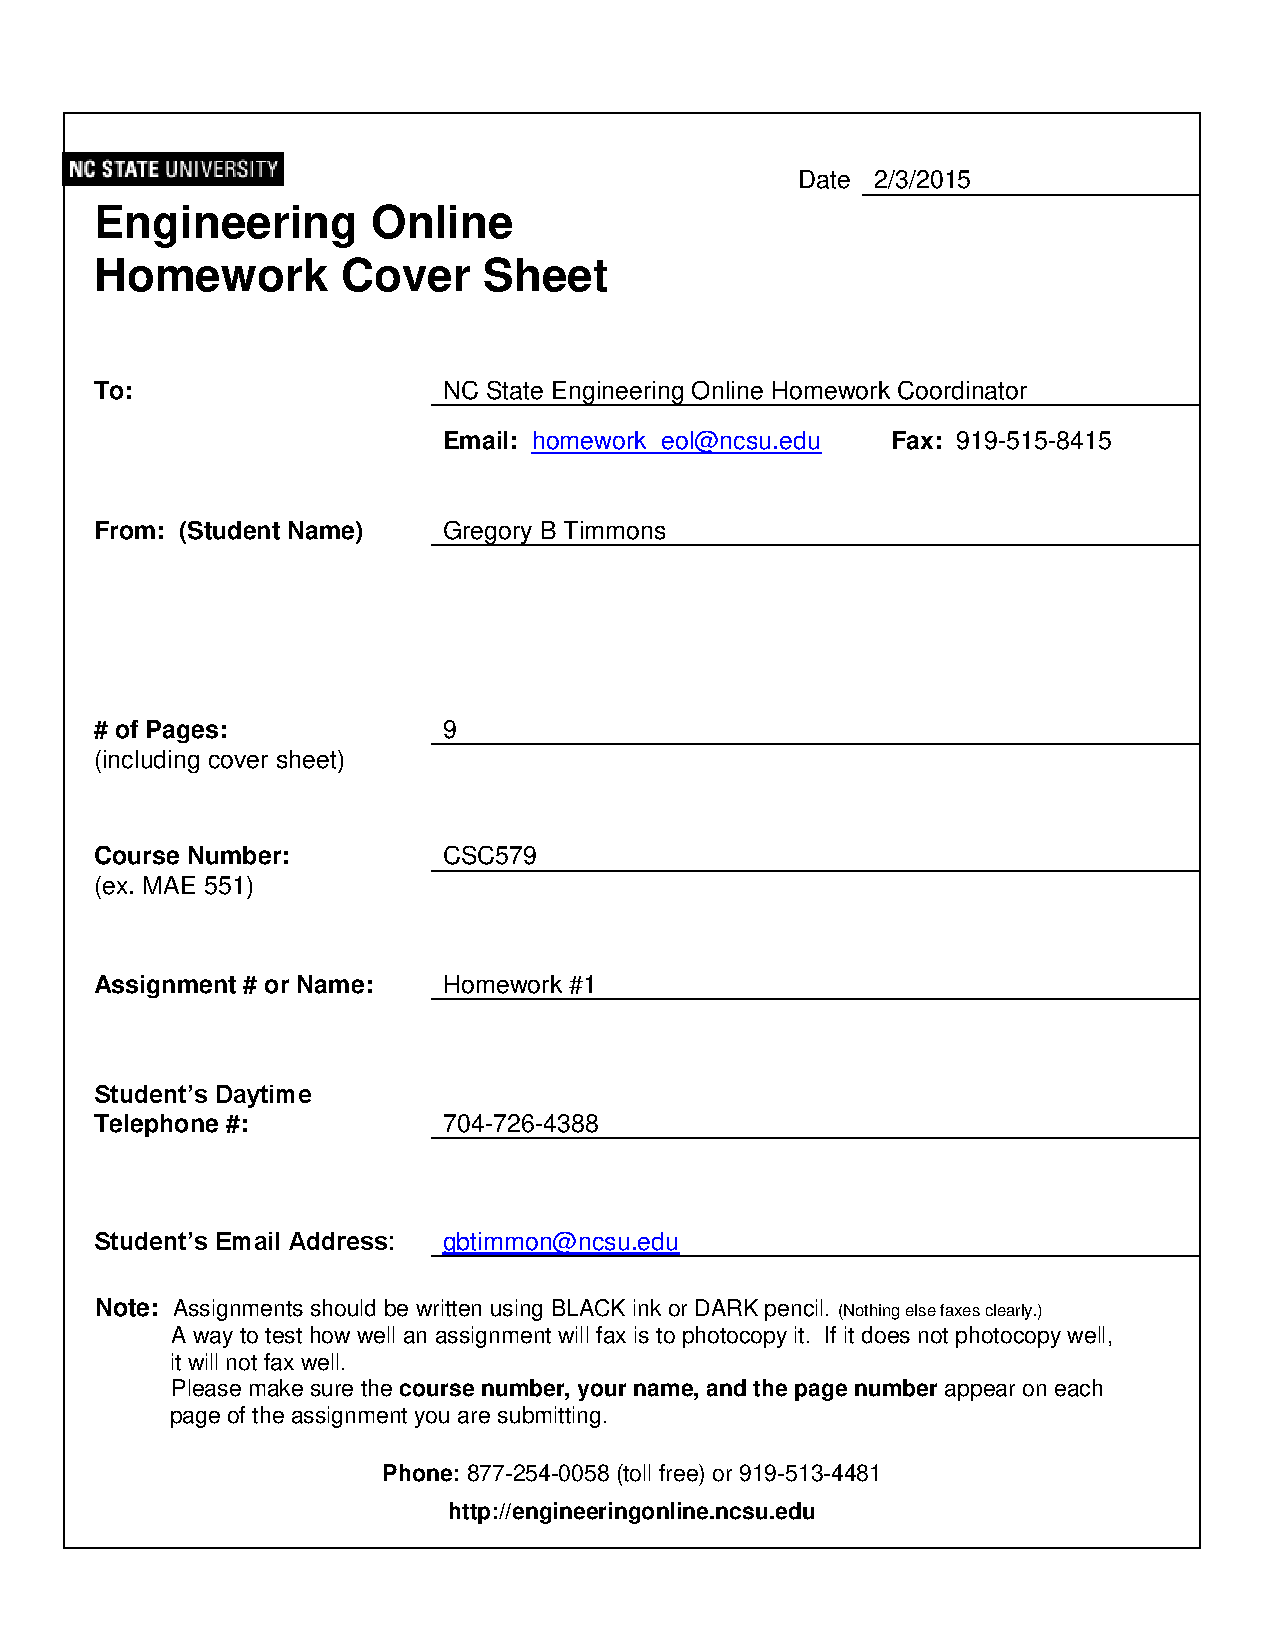
\includepdf[pages={1}]{cover.pdf}
\title{Homework 3}
\date{March 22, 2015}
\author{Gregory B Timmons, gbtimmon}
\maketitle
\section*{Question 1}
\[ P = 
\left(\begin{array}{ccccc}
0.2   & 0.0   & 0.005 & 0.795 & 0.0   \\
0.0   & 0.0   & 0.998 & 0.002 & 0.0   \\
0.002 & 0.0   & 0.0   & 0.0   & 0.998 \\
0.8   & 0.001 & 0.0   & 0.198 & 0.001 \\
0.0   & 0.998 & 0.0   & 0.002 & 0.0   
\end{array}\right)
\]
\\	
\[ P_{HB} = \]\[
\begin{array}{ccccccccccccc}
0.2 &0.005 &0.795 &0.998 &0.002 &0.002 &0.998 &0.8 &0.001 &0.198 &0.001 &0.998 &0.002 \\
1 &3 &4 &3 &4 &1 &5 &1 &2 &4 &5 &2 &4 \\
1 &4 &6 &8 &12 &14 
\end{array}
\]

\[ Q_{HB} = (P^{T} - I)^{T}_{HB} = \]\[
\begin{array}{cccccccccccccccc}
-0.8 &0.005 &0.795 &-1 &0.998 &0.002 &0.002 &-1 &0.998 &0.8 &0.001 &-0.802
&0.001 &0.998 &0.002 &-1 \\
1 &3 &4 &2 &3 &4 &1 &3 &5 &1 &2 &4 &5 &2 &4 &5 \\
1 &4 &7 &10 &14 &17 
\end{array}\]
\section*{Question 2}
The Gauss-Siedel was computed on the Harwell Boeing matrix using the following
matlab code 
\begin{lstlisting}[frame=single] 
 function pi = HW3_gaussSeidel(pi, V, J, I)
    for s = 2 : size(I, 2)  
        sum = 0;
        for i = I(s-1):I(s)-1
            sum = sum + pi(J(i))*V(i);
        end  
        pi(s-1) = sum;
    end
end 
\end{lstlisting}
Using the values \\
$ V = \left(\begin{array}{ccccccc}
	0.4 & 0.6 & 0.4 & 0.4 & 0.2 & 0.2 & 0.8 \\
\end{array}\right)$\\
$ J    = \left(\begin{array}{ccccccc}
	3 & 1 & 2 & 1 & 3 & 3 & 2 \\
\end{array}\right)$\\
$ I   = \left(\begin{array}{cccc}
	1 & 3 & 6 & 8 \\
\end{array}\right)$\\
\\
with \\
$\pi^{(0)} = \left(\begin{array}{ccc}
	0 & 1 & 0
\end{array}\right)$ \\ 
\\
I computed the following values :\\
$\pi^{(1)} = \left(\begin{array}{ccc}
	0  &  0.5556  &  0.4444
\end{array}\right)$ \\ 
$\pi^{(2)} = \left(\begin{array}{ccc}
0.3135   & 0.3407  &  0.3459
\end{array}\right)$ \\ 

\section*{Question 3}
Interarrival time $1/\lambda = .25$ -- mean arrival rate
$\lambda = 4$ \subsection*{(a)}
\[ p_0(t) = e^{-\lambda t}\]
\[ p_{0}(.5) = e^{-(2)} = 0.135 \]
\subsection*{(b)}
At a rate of 4 per hours, we expect to reach ten customers at 2.5 hours. 
\subsection*{(c)}
\[\mbox{Prob}\{N(t) = n \} = p_n(t) = e^{-\lambda t}\frac{(\lambda
t)^{n}}^{n!}\]
\[\mbox{Prob}\{N(.5) > 5 \} = 1 - \mbox{Prob}\{N(.5) \leq 5 \} = 1 -
\sum\limits_{k=0}^{5}p_{k}(.5)\]
\[ =1 - \sum\limits_{k=0}^{5}{e^{-2}\frac{(2)^{n}}^{n!}} = \boxed{0.016}\]
\subsection*{(d)}
Since each customers arrival is uniformly distributed within the hour, both
customers have a $1/6$ independent probability of arriving in the last ten
minutes of the of the hour. Therefore the probability of them both arriving in
this time period is $\boxed{1/6^2}$
\subsection*{(e)}	
\[ 1/6 + 5/6*1/6 = \boxed{11/6^2}\]
\section*{Question 4}
\[ \rho = \frac{\lambda}{\mu}, \quad \rho = .8, \quad \mu = 2 \quad \Rightarrow
\lambda = 1.6\]
Although it is not explicit in the question I will make the assumption that the
2.5 minutes waiting for service is an \underline{average} queue time, that is : 
\[W_q = 2.5, \quad \boxed{R = 3} \]
Littles law state the average number is the system is 
\[L = \lambda W, \quad \boxed{L = 4.8}\]
\newpage
\section*{Question 5}
\[\lambda = 10, \quad \mu = 15, \quad \rho = \frac{\lambda}{\mu} = \frac{2}{3}
\]
\subsection*{(a)}
\[ p_0 = 1 - \rho = \boxed{1/3} \]
\subsection*{(b)}
\[ L_q = \frac{\rho^2}{1 - \rho} = \frac{\left(2/3\right)^2}{1 -
\left(2/3\right)} = \boxed{4/3}
\]
\subsection*{(c)}
\[E[R]= \frac{1}{\mu - \lambda} = \frac{1}{15 - 10} = \boxed{1/5  \quad
\mbox{*(12 minutes)}}\]

\subsection*{(d)}
\[0.125 = \frac{1}{\mu - 10} \Rightarrow 0.125\mu - 1.25 = 1 \Rightarrow
\boxed{\mu = 18 }\
\]

\subsection*{(e)}
\[(1-\rho) * 24  = \boxed{\mbox{ 8 papers an hour}}\]

\section*{Question 6}
\[\mu = 4, \quad W_q = .2 \mbox{ or 12 minutes}\]
\[.2 = \frac{\lambda}{4(4-\lambda)} \Longrightarrow \boxed{ \lambda = 16/9} \]

\section*{Question 7}
\[ \lambda = 3, \quad \mu = 7.5, \quad \rho = 0.4 \]

\subsection*{(a)}
\[\boxed{ \rho = 0.4 }\]
since if the service is being utilize they will have to wait and this is the
average utilization. 
\subsection*{(b)}
\[L_q = \frac{\rho^2}{1-\rho} = \frac{0.4^2}{1-0.4} = \boxed{4/15}\]
\subsection*{(c)}
\[\mbox{Prob}\{N > 5\} = 1 - \mbox{Prob}\{N \leq 5\}\]
\[= 1 -\sum\limits_{n=0}^{5}p_n = 1 - \sum\limits_{n=0}^{5}{\rho^n(1 -
\rho)}\]\[ = 1 - \sum\limits_{k=0}^{5}{0.4^k(1 -
0.4)} = \boxed{0.004096} \]
\subsection*{(d)}
\[W_q(t) = 1 - \rho e^{\mu (1- \rho)t} \]
\[\mbox{Prob}\{\mbox{Wait time} \leq \mbox{12 mins} | \mbox{the server is busy}
\} = W_q(0.20) = 1 - 0.4 e^{-7.5 (1- 0.4).20} = 0.8373 \] \[\mbox{Prob}\{
\mbox{Wait time} > \mbox{12 mins} \} = 0.6 + 0.4(0.8373) = \boxed{0.9349}\]
\subsection*{(e)}
\[8/60 = \frac{\lambda}{7.5(7.5 - \lambda)}\quad \Rightarrow \boxed{\lambda =
3.75}}\]

\section*{Question 8}


\subsection*{(a)}
Yes the Pasta therom does hold $p_n = a_n$. The probabitlity of seeing a certain
number in the system for a particular arrival is the same as the probility of
the system holding that many people at equlibrium.
\subsection*{(b)} We are
concerned with weather or not we have unbounded growth of the queue. In a normal queue if $\rho > 1$ the rate of arrivals is greater then the rate of exit
from the system and the growth of the queue will be unbounded. Since the rate of
arriavl is dependent on n, then the arrival rate slows and we will always bound
our queue. Any $\boxed{\rho < \infty}$ should be sufficent to bound the size of
the queue and ensure the stability of the queue.
\\

Put mathmatically : 
\[\left[\sum_{n=0}^{\infty}{\left(\frac{\rho^n}{n!}\right)}}\right]\]
(as derived below) Converges for any $\rho$, therefor the system will remain
stable for any $\rho < \infty$.
 \subsection*{(c)}
Assuming $\rho < \infty$ 
\[ p_n = p_0\prod_{i=0}^{n-1}{\frac{\lambda}{\mu(n + 1)}} =
p_0\left(\frac{\rho^n}{n!}\right)	
\]
\[ 1 = \sum_{n=0}^{\infty}{p_n} =
\sum_{n=0}^{\infty}{p_0\left(\frac{\rho^n}{n!}\right)}}\] 
	\[p_0 = \left[\sum_{n=0}^{\infty}{\left(\frac{\rho^n}{n!}\right)}}\right]^{-1}
	= e^{-\rho}\]
\[\boxed{p_n = \left(\frac{\rho^n}{n!}\right)e^{-\rho}}\] 
\subsection*{(d)}
????
\subsection*{(e)}
\[ L  = E[N] = \sum_{n=0}^{\infty}np^n =
\sum_{n=0}^{\infty}n\left(\frac{\rho^n}{n!}\right)e^{-\rho} = \rho \]

\[ \boxed{ L = \rho } \]

\[ R_n = \frac{\frac{\lambda}{n+1}p_n}{\sum_{k=0}^{\infty}p_k}
=
\frac{\frac{\rho^{n+1}}{(n+1)!}e^{-\rho}}{\sum_{k=0}^{\infty}{\frac{\rho^{k+1}}{(k+1)!}e^{-\rho}}}
= \frac{p_{n+1}}{1 - e^{-\rho}}\]
\[E[R] = \sum_{k=0}^{\infty}{\frac{k+1}{\mu}R_k}} =
\frac{1}{\mu}\sum_{k=0}^{\infty}{\frac{(k+1)p_{k+1}}{1 - e^{-\rho}}} =
\frac{1}{\mu(1-e^{-\rho})}L = \frac{\rho}{\mu(1-e^{-\rho})}\]
\[\boxed{R = \frac{\rho}{\mu(1-e^{-\rho})}}}\]
\\
\\
The following source was use in answering this
question:\\http://irh.inf.unideb.hu/\~jsztrik/education/16/SOR\_Main\_Angol.pdf \section*{Question 9}
This is an example of an M/M/5 or M/M/6 queue respectively.
\[ \mbox{ 6/3/5 } : \lambda = 6, \quad \mu = 3, \quad c = 5, \quad \rho =
\frac{6}{5 * 2} = .6\]

\[ p_0 = 
  \left[ 1 + \left(\sum\limits_{n=1}^{c-1}{\frac{(c\rho)^n
  }{n!}}\right) + \frac{(c\rho)^c}{c!}\frac{1}{1 - \rho}\right]^{-1}\]

\[ p_0 = 
  \left[ 1 + \left(\sum\limits_{n=1}^{5-1}{\frac{(5 * .6)^n
  }{n!}}\right) + \frac{(5 * .6)^5}{5!}\frac{1}{1 - .6}\right]^{-1}\]
  
\[ \boxed{p_0 = 0.0466472} \]


\[ W_q = \left[
\frac{(\lambda/\mu)^c\mu}{(c - 1)!(c\mu - \lambda)^2} \right]p_0 \] 

\[W_q = \left[\frac{3(6/3)^5}{(5 - 1)!(5(3) - 6)^2}\right] * 0.0466472\]

\[ W_q = 0.0023032 \mbox{ hours } , \boxed{8.29 \mbox{ seconds}}\]
This should satisfy the requirement. 
\[ \mbox{ 6/3/6 } : \lambda = 6, \quad \mu = 3, \quad c = 6, \quad \rho =
\frac{6}{6 * 2} = .5\]

\[ p_0 = 
  \left[ 1 + \left(\sum\limits_{n=1}^{c-1}{\frac{(c\rho)^n
  }{n!}}\right) + \frac{(c\rho)^c}{c!}\frac{1}{1 - \rho}\right]^{-1}\]

\[ p_0 = 
  \left[ 1 + \left(\sum\limits_{n=1}^{5-1}{\frac{(5 * .5)^n
  }{n!}}\right) + \frac{(5 * .5)^5}{5!}\frac{1}{1 - .5}\right]^{-1}\]
  
\[ \boxed{p_0 = 0.0801001} \]


\[ W_q = \left[
\frac{(\lambda/\mu)^c\mu}{(c - 1)!(c\mu - \lambda)^2} \right]p_0 \] 

\[W_q = \left[\frac{3(6/3)^6}{(6 - 1)!(6(3) - 6)^2}\right] * 0.0801001\]

\[ W_q = 0.00089 \mbox{ hours } , \boxed{3.2 \mbox{ seconds}}\]
 \section*{Question 10}
 \[10/20/1/2 : \quad \lambda = 10, \quad \mu = 20, \quad \rho = .5 , \quad k =
 2.\] 
 \subsection*{(a)}
 \[p_n = \frac{(1-\rho)\rho^n}{1-\rho^{K+1}}\]
 \[p_0 = \frac{(1-.5)}{1-.5^3} = \boxed{0.571429}\]
 \[p_1 = \frac{(1-.5).5}{1-.5^3} = \boxed{0.285714}\]
 \[p_2 = \frac{(1-.5).5^2}{1-.5^3} = \boxed{0.142857}
 \]
 \subsection*{(b)}
 \[ \mbox{ Throughput }X = \lambda ( 1 - p_2) \]
 \[ X = 10(1 - 0.142857) = 8.57143 \] 
 \[\mbox{ Utilization } U = \frac{1}{\mu}X  = \frac{1}{20}8.57143 \]
 \[ U = 42.85\% \] 
 The server is busy $\boxed{42.85\%}$ of the time. 
 In 8 hours the servers throughput is 8.57 an hour therefor he should server
 $\boxed{68.5}$ people
  \subsection*{(c)}
  If 10 customers arrive and hour and 8.57143 get serviced on average then
  $\boxed{85.7143\%}$ of customers succed in getting their shoes shined and
  $(100 - 85.7143)\%$ will get turned away. 
  
\end{document}
